\documentclass[12pt]{article}
%DIF LATEXDIFF DIFFERENCE FILE
%DIF DEL revision/rom_sciAdvances_rev.tex     Thu Dec 20 11:40:11 2018
%DIF ADD revision2/rom_sciAdvances_rev2.tex   Tue Jan 29 17:33:28 2019

\usepackage{scicite}
\let\citep=\cite

% \usepackage{times}


\usepackage{graphicx}
\usepackage{authblk}
\usepackage{lineno}
\usepackage{paralist}
\usepackage{amsmath}

\topmargin 0.0cm
\oddsidemargin 0.2cm
\textwidth 16cm 
\textheight 21cm
\footskip 1.0cm


% environment for the abstract
\newenvironment{sciabstract} 
{\bfseries}
{}


\title{Non-equilibrium evolution of volatility in origination and
  extinction explains fat-tailed fluctuations in Phanerozoic
  biodiversity \\
  \vspace{1em} \large {\it One sentence summary:} Phanerozoic marine
  invertebrate richness fluctuates out of equilibrium due to pulsed
  adaptive evolution.}

\author[1, {*}]{Andrew J. Rominger}
\author[1, 2, 3]{Miguel A. Fuentes}
\author[1, 4, 5, 6, 7, 8]{Pablo A. Marquet}

\affil[1]{\normalsize{Santa Fe Institute, 1399 Hyde Park Road, Santa Fe, New
Mexico 87501, US}}
%
\affil[2]{\normalsize{Instituto de Investigaciones Filos\'oficas, SADAF, CONICET,
Bulnes 642, 1428 Buenos Aires, Argentina}}
%
\affil[3]{\normalsize{Facultad de Ingenier\'ia y Tecnolog\'ia, Universidad San
Sebasti\'an, Lota 2465, Santiago 7510157, Chile}}
%
\affil[4]{\normalsize{Departamento de Ecolog\'ia, Facultad de Ciencias
Biol\'ogicas, Pontificia Universidad de Chile, Alameda 340, Santiago,
Chile}}
%
\affil[5]{\normalsize{Instituto de Ecolog\'ia y Biodiversidad (IEB),
    Casilla 653, Santiago, Chile}}
%
\affil[6]{\normalsize{Laboratorio Internacional de Cambio Global
    (LINCGlobal), and Centro de Cambio Global UC, Pontificia
    Universidad Catolica de Chile, Santiago, Chile.}}
%
\affil[7]{\normalsize{Instituto de Sistemas Complejos de Vlapara\'iso
    (ISCV), Artiller\'ia 470, Cerro Artiller\'ia, Valpara\'iso,
    Chile}}
%
\affil[8]{\normalsize{Centro de Ciencias de la Complejidad (C3),
    Universidad Nacional Aut\'onoma de M\'exico.}}
%
\affil[{*}]{\normalsize{To whom correspondence should be addressed,
    e-mail: rominger@santafe.edu}}

\date{}



%%%% END OF PREAMBLE %%%%
%DIF PREAMBLE EXTENSION ADDED BY LATEXDIFF
%DIF UNDERLINE PREAMBLE %DIF PREAMBLE
\RequirePackage[normalem]{ulem} %DIF PREAMBLE
\RequirePackage{color}\definecolor{RED}{rgb}{1,0,0}\definecolor{BLUE}{rgb}{0,0,1} %DIF PREAMBLE
\providecommand{\DIFadd}[1]{{\protect\color{blue}\uwave{#1}}} %DIF PREAMBLE
\providecommand{\DIFdel}[1]{{\protect\color{red}\sout{}}}                      %DIF PREAMBLE
%DIF SAFE PREAMBLE %DIF PREAMBLE
\providecommand{\DIFaddbegin}{} %DIF PREAMBLE
\providecommand{\DIFaddend}{} %DIF PREAMBLE
\providecommand{\DIFdelbegin}{} %DIF PREAMBLE
\providecommand{\DIFdelend}{} %DIF PREAMBLE
%DIF FLOATSAFE PREAMBLE %DIF PREAMBLE
\providecommand{\DIFaddFL}[1]{\DIFadd{#1}} %DIF PREAMBLE
\providecommand{\DIFdelFL}[1]{\DIFdel{#1}} %DIF PREAMBLE
\providecommand{\DIFaddbeginFL}{} %DIF PREAMBLE
\providecommand{\DIFaddendFL}{} %DIF PREAMBLE
\providecommand{\DIFdelbeginFL}{} %DIF PREAMBLE
\providecommand{\DIFdelendFL}{} %DIF PREAMBLE
\newcommand{\DIFscaledelfig}{0.5}
%DIF HIGHLIGHTGRAPHICS PREAMBLE %DIF PREAMBLE
\RequirePackage{settobox} %DIF PREAMBLE
\RequirePackage{letltxmacro} %DIF PREAMBLE
\newsavebox{\DIFdelgraphicsbox} %DIF PREAMBLE
\newlength{\DIFdelgraphicswidth} %DIF PREAMBLE
\newlength{\DIFdelgraphicsheight} %DIF PREAMBLE
% store original definition of \includegraphics %DIF PREAMBLE
\LetLtxMacro{\DIFOincludegraphics}{\includegraphics} %DIF PREAMBLE
\newcommand{\DIFaddincludegraphics}[2][]{{\color{blue}\fbox{\DIFOincludegraphics[#1]{#2}}}} %DIF PREAMBLE
\newcommand{\DIFdelincludegraphics}[2][]{% %DIF PREAMBLE
\sbox{\DIFdelgraphicsbox}{\DIFOincludegraphics[#1]{#2}}% %DIF PREAMBLE
\settoboxwidth{\DIFdelgraphicswidth}{\DIFdelgraphicsbox} %DIF PREAMBLE
\settoboxtotalheight{\DIFdelgraphicsheight}{\DIFdelgraphicsbox} %DIF PREAMBLE
\scalebox{\DIFscaledelfig}{% %DIF PREAMBLE
\parbox[b]{\DIFdelgraphicswidth}{\usebox{\DIFdelgraphicsbox}\\[-\baselineskip] \rule{\DIFdelgraphicswidth}{0em}}\llap{\resizebox{\DIFdelgraphicswidth}{\DIFdelgraphicsheight}{% %DIF PREAMBLE
\setlength{\unitlength}{\DIFdelgraphicswidth}% %DIF PREAMBLE
\begin{picture}(1,1)% %DIF PREAMBLE
\thicklines\linethickness{2pt} %DIF PREAMBLE
{\color[rgb]{1,0,0}\put(0,0){\framebox(1,1){}}}% %DIF PREAMBLE
{\color[rgb]{1,0,0}\put(0,0){\line( 1,1){1}}}% %DIF PREAMBLE
{\color[rgb]{1,0,0}\put(0,1){\line(1,-1){1}}}% %DIF PREAMBLE
\end{picture}% %DIF PREAMBLE
}\hspace*{3pt}}} %DIF PREAMBLE
} %DIF PREAMBLE
\LetLtxMacro{\DIFOaddbegin}{\DIFaddbegin} %DIF PREAMBLE
\LetLtxMacro{\DIFOaddend}{\DIFaddend} %DIF PREAMBLE
\LetLtxMacro{\DIFOdelbegin}{\DIFdelbegin} %DIF PREAMBLE
\LetLtxMacro{\DIFOdelend}{\DIFdelend} %DIF PREAMBLE
\DeclareRobustCommand{\DIFaddbegin}{\DIFOaddbegin \let\includegraphics\DIFaddincludegraphics} %DIF PREAMBLE
\DeclareRobustCommand{\DIFaddend}{\DIFOaddend \let\includegraphics\DIFOincludegraphics} %DIF PREAMBLE
\DeclareRobustCommand{\DIFdelbegin}{\DIFOdelbegin \let\includegraphics\DIFdelincludegraphics} %DIF PREAMBLE
\DeclareRobustCommand{\DIFdelend}{\DIFOaddend \let\includegraphics\DIFOincludegraphics} %DIF PREAMBLE
\LetLtxMacro{\DIFOaddbeginFL}{\DIFaddbeginFL} %DIF PREAMBLE
\LetLtxMacro{\DIFOaddendFL}{\DIFaddendFL} %DIF PREAMBLE
\LetLtxMacro{\DIFOdelbeginFL}{\DIFdelbeginFL} %DIF PREAMBLE
\LetLtxMacro{\DIFOdelendFL}{\DIFdelendFL} %DIF PREAMBLE
\DeclareRobustCommand{\DIFaddbeginFL}{\DIFOaddbeginFL \let\includegraphics\DIFaddincludegraphics} %DIF PREAMBLE
\DeclareRobustCommand{\DIFaddendFL}{\DIFOaddendFL \let\includegraphics\DIFOincludegraphics} %DIF PREAMBLE
\DeclareRobustCommand{\DIFdelbeginFL}{\DIFOdelbeginFL \let\includegraphics\DIFdelincludegraphics} %DIF PREAMBLE
\DeclareRobustCommand{\DIFdelendFL}{\DIFOaddendFL \let\includegraphics\DIFOincludegraphics} %DIF PREAMBLE
%DIF END PREAMBLE EXTENSION ADDED BY LATEXDIFF

\begin{document} 


\newcommand{\beginsupplement}{%
  \setcounter{table}{0}
  \renewcommand{\thetable}{S\arabic{table}}%
  \setcounter{figure}{0}
  \renewcommand{\thefigure}{S\arabic{figure}}%
  \setcounter{section}{0}
  \renewcommand{\thesection}{S\arabic{section}}%
}

\beginsupplement

\begin{center}
{\LARGE \bf Supplementary materials}
\end{center}
\vspace{2em}

\section{Limit distribution of a time-averaged homogeneous
  origination-extinction process}
\label{sec:suppLimitDist}

Fossil taxa gain and lose genera according to an
origination-extinction process. We, however, do not see every event of
this processes but rather a time average imposed by the coarse
resolution of the rock record. In our analysis we use time bins of
approximately 11 MY and it is over this duration that the history of
originations and extinctions are time-averaged resulting in observed
taxon richnesses and fluctuations thereof. Such time-averaged Markov
processes have already been shown to be asymptotically
Gaussian\citep{grassmann1987}.  Using the asymptotic Gaussian
approximation is also a more appropriate distribution for our sampling
and bias-corrected richness estimates because these estimates are not
integer-valued but rather continuous random variables.


What is more, because preservation and sampling are far from complete
we likely only recover taxa when they are in an abundant and largely
stationary period in their macroevolution \citep{liow2007}. This
stationarity gives us another lens on the asymptotic normality of
fluctuations because average per capita rates of origination and
extinction would be equal (i.e.  $\lambda = \mu \equiv \rho$) over a
coarse-grained interval of duration $\tau$ and the number of
origination or extinctions events (call such events $Y$) each follow
an inhomogeneous Poisson process with rate $\tau \rho N_t$. Here $N_t$
is the time-averaged number of genera in the taxon of interest during
the interval of length $\tau$ at time $t$.

The difference of these Poisson distributions is again asymptotically
Gaussian.  Our analysis does not depend on all clades being perfectly
stationary with $\lambda = \mu$ because of the asymptotics of
time-averaged Markov processes. Indeed we zero-center all fluctuation
time series to avoid possible net diversification or extinction from
biasing our analysis of fluctuation volatilities.


\section{Evaluation of sampling bias correction methods}
\label{sec:suppBiasEval}

Our sampling and bias-correction method first accounts for imperfect
detection within a binomial sampling framework as described in the
main text, and then further corrects for potential publication bias
using simple log-log regression.  We reproduce that regression of
log-richness versus log-number of publications here
(Fig. \ref{figSupp:divByPub}). 

\begin{figure}[!hp]
  \centering
  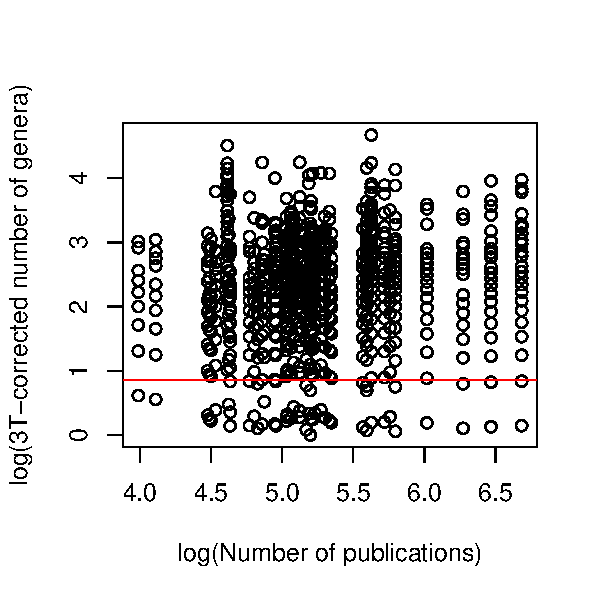
\includegraphics[width=0.4\textwidth]{../../figSupp_divByPub.pdf}
  \caption{Relationship between number of publications and three-timer
    (3T) corrected genus richness at the family level as recorded by
    the PBDB.}
  \label{figSupp:divByPub}
\end{figure}


We compare our sampling and bias-correction method to other more
established approaches. Specifically we use the newly available R
package {\it divDyn} \citep{kocsis2018} to produce subsampling-based
richness estimates for the Phanerozoic timeseries of marine
invertebrates. In Figure \ref{figSupp:3TPub} we compare classical
rarefaction and shareholder quorum subsampling (SQS) with our
method. All samples were rarified to 120 occurrences, which is
approximately the maximum possible rarefied sample size across all
time bins, and the SQS quorum was set to 0.75 to similarly approximate
this common sampling denominator across time bins. For both
rarefaction and SQS we averaged 50 subsampled replicates.

  
\begin{figure}[!hp]
  \centering
  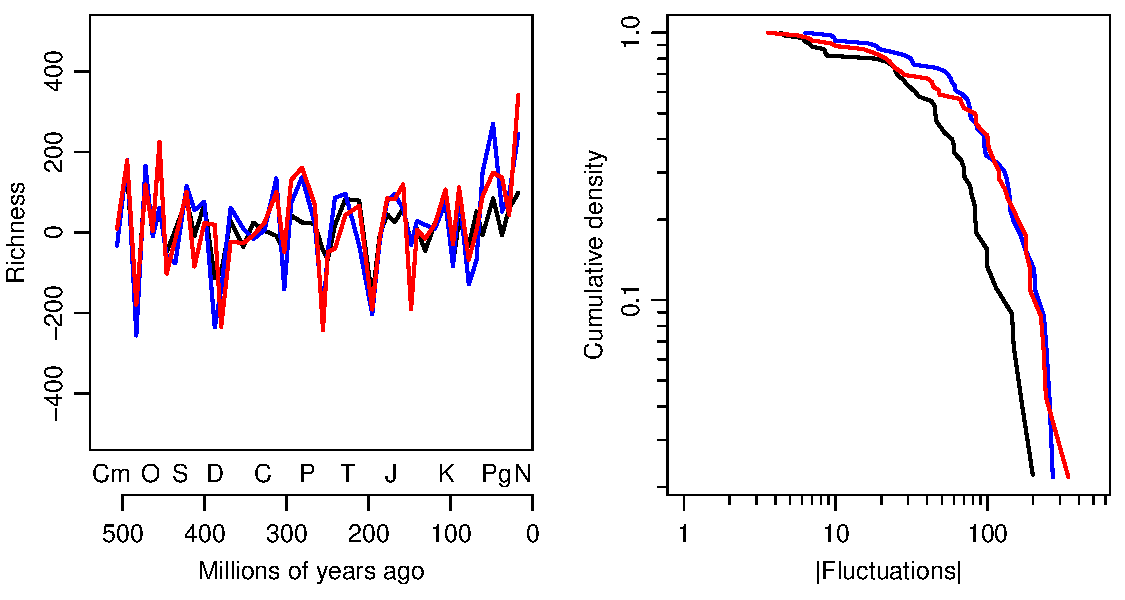
\includegraphics[width=0.7\textwidth]{../../figSupp_divEstComp.pdf}
  \caption{Comparison of rarefaction (black line) and SQS (blue)
    with our three-timer and publication bias correction method
    (red). The time-series of all marine invertebrate genera shows
    general agreement with the only major deviations toward the modern
    (A). Despite these differences the distribution of fluctuations in
    genus richness across all marine invertebrates show good agreement
    (B).}
  \label{figSupp:3TPub}
\end{figure}


\section{Understanding deviations from superstatistics at higher
  taxonomic levels}
\label{sec:suppSstatTaxLevels}

To explore why deviations from super statistics increase with
increasing taxonomic level we explore how the distributions of
richness fluctuations $p_k(x | \beta_k)$ and fluctuation volatilities
$f(\beta_k)$ change with changing taxonomic level. We find that
richness fluctuation distributions experience increasing frequencies
of outliers (increasing kurtosis) with higher taxonomic level
(Fig. \ref{figSupp:pkx_allTaxa}). We also find that observed
fluctuation volatility distributions increasingly depart from a Gamma
distribution at the levels of classes and phyla
(Fig. \ref{figSupp:fbeta_allTaxa}).

\begin{figure}[!hp]
  \centering
  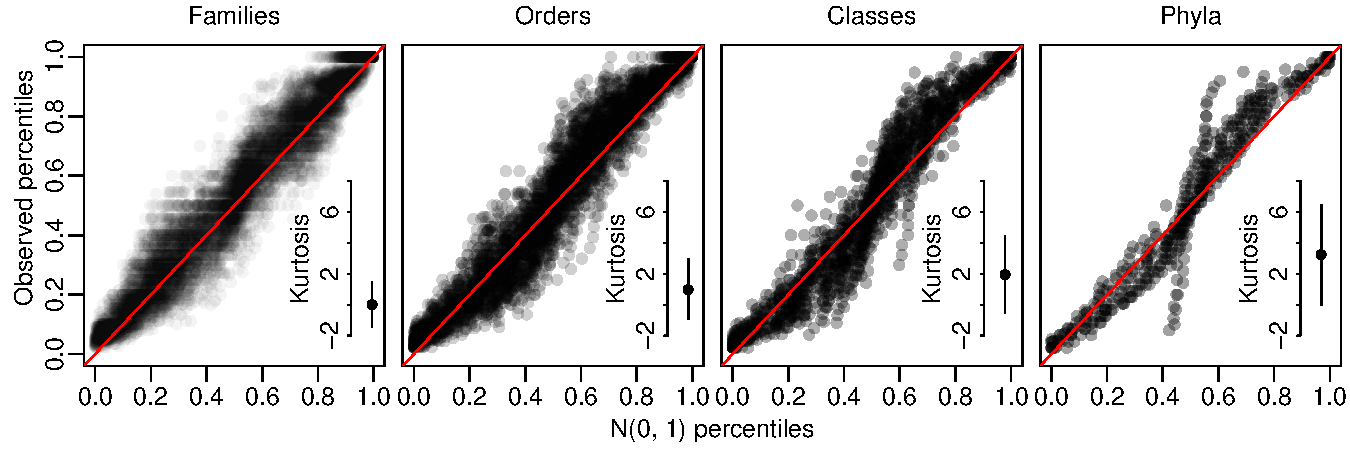
\includegraphics[width=0.8\textwidth]{../../figSupp_pkx_allTaxa.pdf}
  \caption{Change in within clade richness fluctuation distributions
    with increasing taxonomic level. The percentile-percentile plots
    show how the percentiles of observed re-scaled fluctuation
    distributions compare to expected percentiles from a Gaussian
    distribution with mean 0 and variance 1. We can see that families
    and order conform to a linear relationship, albeit with the later
    showing some signs of an s-shaped pattern. Clases and phyla show
    stronger deviations from the linear trend with a marked s-shaped
    relationships. Inset plots show how kurtosis increases from 0 (the
    value for a Gaussian distribution) at the family level to
    increasingly larger values at higher taxonomic levels.}
  \label{figSupp:pkx_allTaxa}
\end{figure}

\begin{figure}[!hp]
  \centering
  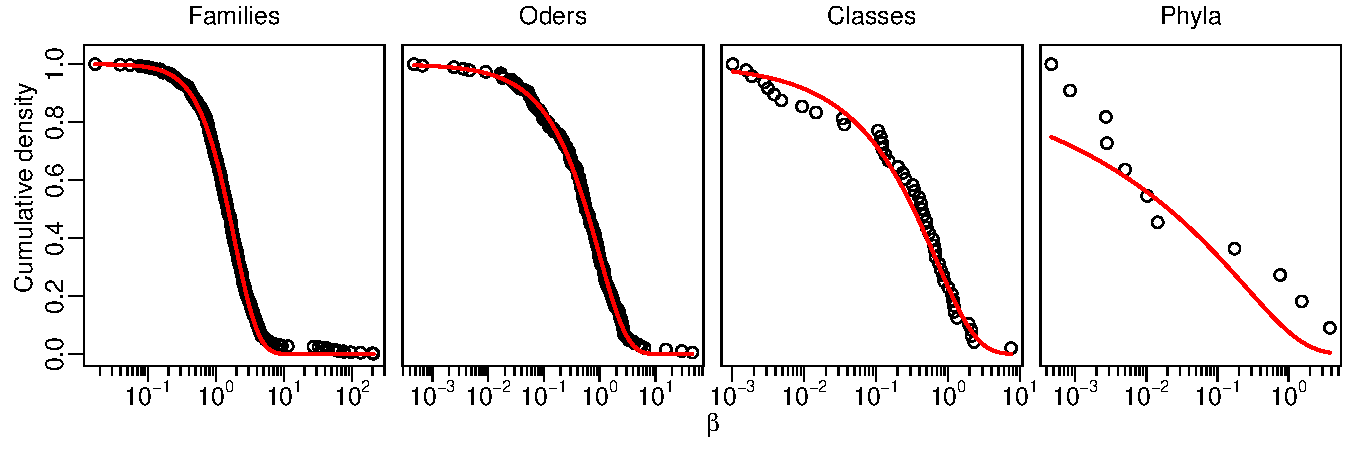
\includegraphics[width=0.8\textwidth]{../../figSupp_fbeta_allTaxa.pdf}
  \caption{Change in the distributions of $\beta_k$ across clades of
    increasing taxonomic level. Points are observed $\beta_k$ values
    and red lines are the best-fit Gamma distributions. Deviations
    increase particularly at the class and phylum levels.}
  \label{figSupp:fbeta_allTaxa}
\end{figure}


\section{Ecospace occupation of higher taxa}
\label{sec:suppGuilds} 

We posit that part of the increasing divergence between
superstatistics and observed fluctuations and the increase in
fluctuation outliers at higher taxonomic levels is that these higher
taxa increasingly aggregate disparate types of organisms. One way to
evaluate this idea is to count the ecospace hypercubes
\citep{bambach1983, bambach2007, bush2007} occupied by taxa at
different levels. We use the ecological characteristics reported by
the PBDB: taxon environment, motility, life habit, vision, diet,
reproduction, and ontogeny. In Figure \ref{figSupp:eeSpaceOcc} we find
that families comprise, on average, 1 hypercube, orders comprise 2
hypercubes on average, and classes and phyla comprise many more.

\begin{figure}[!hp]
  \centering
  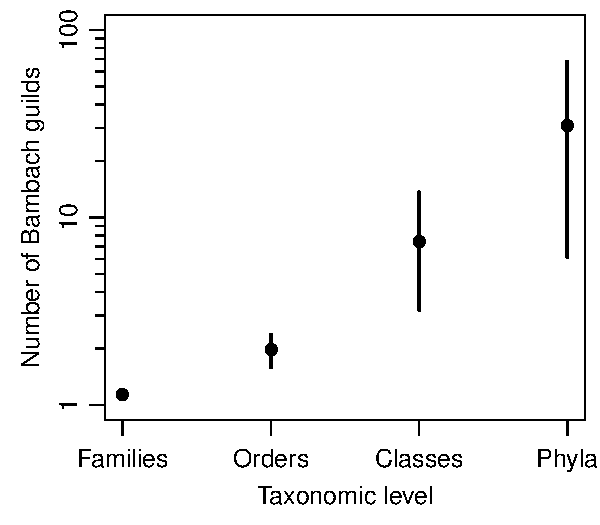
\includegraphics[width=0.4\textwidth]{../../figSupp_eeSpaceOcc.pdf} 
  \caption{Relationship between number of ecospace hypercubes occupied
    and taxonomic level.}
  \label{figSupp:eeSpaceOcc}
\end{figure}


\section{Relationship between $\beta_k$ and clade richness}
\label{sec:suppBetaRichness} 

There is likely to be a relationship between richness of clade $k$ and
its fluctuation volatility $\beta_k$ because both extinction and
origination (i.e. the formation of new genera) contribute to
volatility. Thus we expect that higher variance in richness
fluctuations (i.e. smaller $\beta_k = 1/\text{variance}$) will be
correlated with higher richness.  Indeed, Figure
\ref{figSupp:betaByRich} shows this to be true. 

\begin{figure}[!hp]
  \centering
  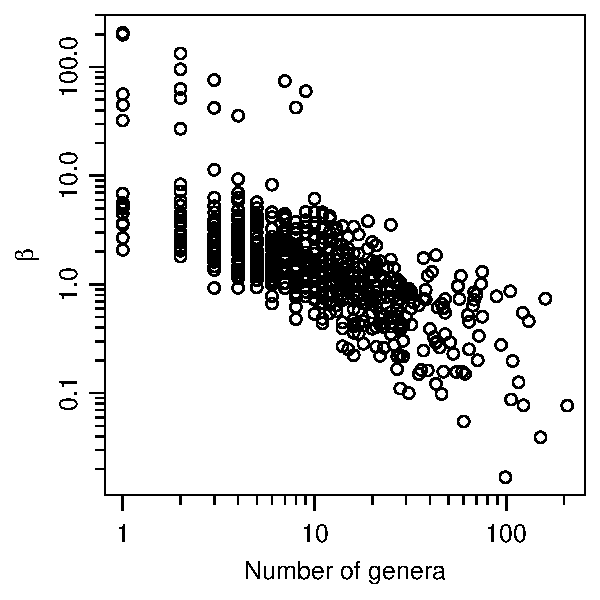
\includegraphics[width=0.4\textwidth]{../../figSupp_betaByRich.pdf} 
  \caption{Relationship between fluctuation volatility $\beta_k$ and
    genus richness at the family level.}
  \label{figSupp:betaByRich}
\end{figure}

In the main text we use permutation to evaluate whether this
correlation is responsible for the observed good fit of
superstatistics, and find that this correlation alone is not
sufficient. \DIFaddbegin \DIFadd{In addition to this permutation test,
  we directly evaluate whether the distribution of clade richness at
  the family level conforms to a Gamma distribution
  (Fig. \ref{figSupp:richGamma}). If the family-level richness
  distribution had mirrored the distribution of $\beta_k$ values this
  may have suggested that richness was largely responsible for
  superstatistical behavior. However, we find that family richness is
  not Gamma (Fig. \ref{figSupp:richGamma}), reaffirming the
  permutation-based findings that the $\beta_k$ values derive from
  more nuanced biological mechanisms.}\DIFaddend

\begin{figure}[!hp]
  \centering
  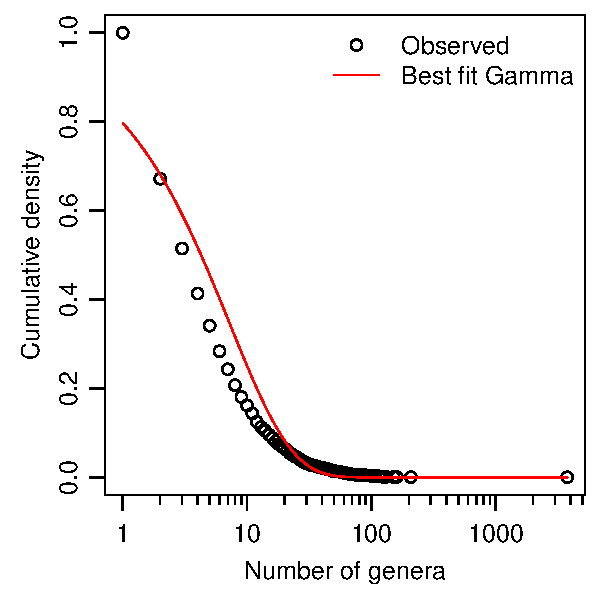
\includegraphics[width=0.4\textwidth]{../../figSupp_richGamma.pdf} 
  \caption{Distribution of genus richnesses within families. Red line
    shows best-fit Gamma distribution which clearly deviates from the
    observed cumulative density function (black points).}
  \label{figSupp:richGamma}
\end{figure}

\end{document}

